\section{BusyBox简介}
\subsection{简单介绍}

\begin{figure}[htb]
	\centering
	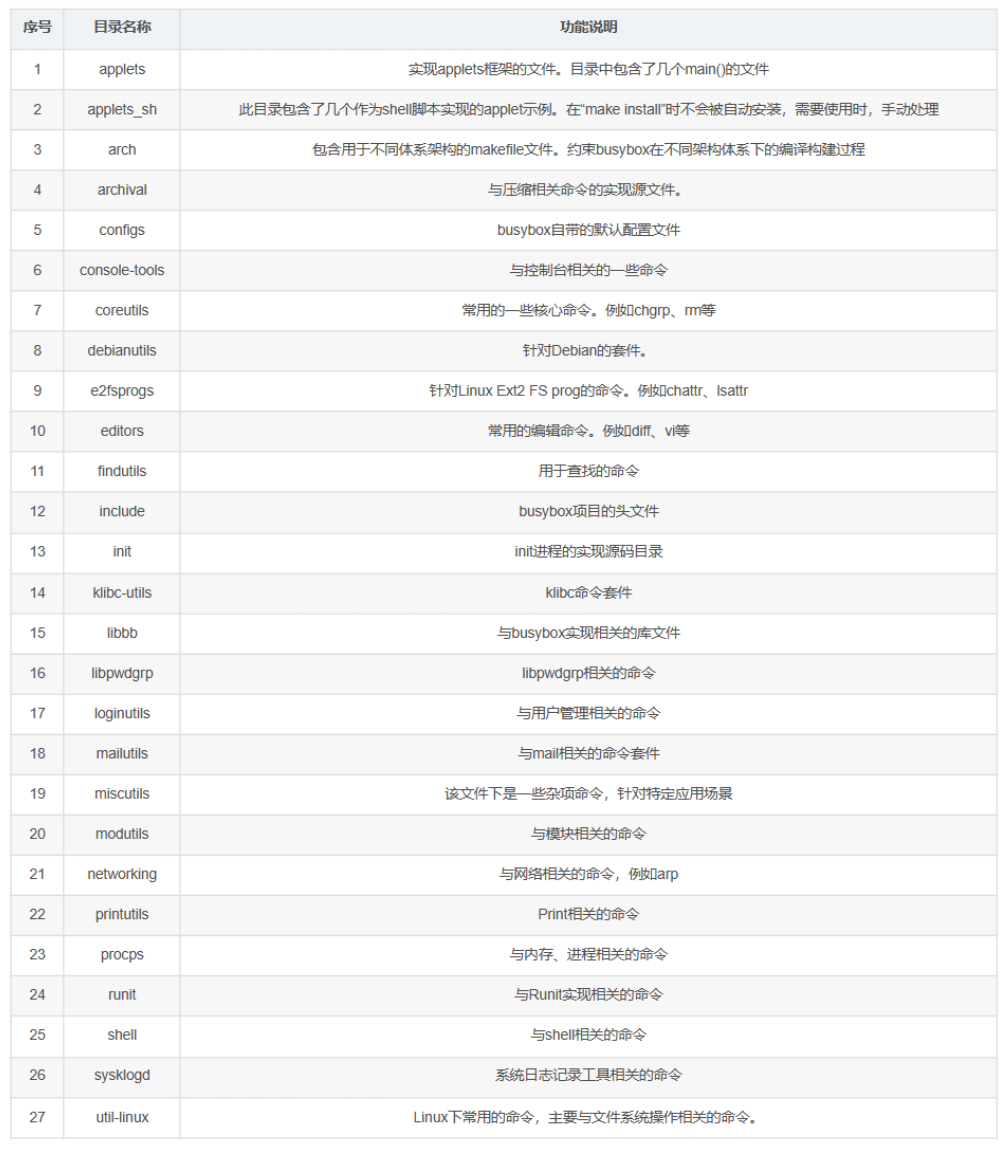
\includegraphics[width=\textwidth]{figures/09-02-Busybox源码目录结构.png}
	\caption{
		Busybox源码目录结构
	}
	\label{fig:user virtual process}
\end{figure}

BusyBox是一个针对嵌入式系统的轻量级工具集合,旨在通过整合常用的
Linux命令和服务程序,将它们合并为一个单一的可执行文件。这个项目
最初于1996年诞生,当时嵌入式系统并不像今天这般普及。BusyBox的
最初目的是为软盘系统设计的,因为在那个时候,可移动存储介质的容
量十分有限,软盘是主要的存储媒介之一。

BusyBox的设计理念非常巧妙。相较于单独存放每个命令所需的存储空间
,BusyBox通过将不同命令的共享部分整合到一起,极大地减小了可执行
文件的体积。举例来说,诸如grep和find这样的命令,尽管功能有所差
异,但它们都需要从文件系统中搜索文件,BusyBox将这部分代码进行
共享,从而节省了空间。

BusyBox的核心特点在于其高度紧凑的特性。它可以包含最基本的系统
命令,例如文件列表显示命令ls和文件内容查看命令cat,同时也能整
合更复杂的程序,如文本搜索命令grep和文件查找命令find,甚至还
能将HTTP服务器整合进同一个软件包中。

对于嵌入式系统来说,存储空间十分宝贵,而BusyBox的存在则为这些
系统提供了解决方案。通常情况下,BusyBox的可执行文件大小仅约1MB
左右,相比于分散存放各个命令所需的存储空间,这是一个相当节省空间
的选择。用户可以通过建立链接的方式,与传统的命令一样使用BusyBox
,只不过它将多个功能整合到一个文件中,从而在嵌入式系统中占用更少
的存储空间。

Busybox源码目录结构图如上,方便以后对Busybox做裁剪的时候参考。

\subsection{工作原理}
BusyBox利用了shell传递给C语言main()函数的参数,回想一下C语言
main()函数的定义:int main(int argc,char *argv[])

在main()函数的定义中argc是传递进来的参数个数,argv是一个字符串
数组,数据的每一项都是一个参数内容。其中,argv[0]是从命令行调用
的程序名。下面是一个简单的程序,使用argv[0]确定调用来自哪个程序
。

\begin{lstlisting}[language=Rust]
	//test.c
	#include <stdio.h>
	/*定义主函数*/
	int main(int argc,char *argv[])
	int i;
	for(i=0;i<argc ;i++){
		//for循环语句
		printf("argv[8d]=8s\n",i,argv[i]);//打印程序参数内容
	 }
	return 0;
    }
\end{lstlisting}

调用这个程序会显示所调用的第一个参数是该程序的名字。可以对这个可执行程序重新进行命名,此时再调用就会得到该程序的新名字。另外,可以创建一个到可执行程序的符号链接,在执行这个符号链接时,就可以看到这个符号链接的名字。

\begin{lstlisting}[language=Rust]
	$  gcc -Wall -o test test.c
	$  ./test argl arg2
	argv[0]=./test
	argv[1]=arg1
	argv[2]=arg2

	$  mv test newtest
	$  ./newtest argl
	argv[0]=./newtest
	argv[1]=arg1

	$  ln -s newtest linktest
	$  ./linktest arg
	argv[0]=./linktest
	argv[1]=arg
	\end{lstlisting}

BusyBox使用符号链接屏蔽了程序调用细节。从用户的角度看,使用BusyBox与使用传统的命令效果是相同的。BusyBox为其包含的每个系统程序都建立了类似的符号链接。当用户使用符号链接调用BusyBox的时候,BusyBox通过argv[0]参数调用对应的功能函数。

\subsection{使用方法}
\subsubsection{BusyBox初始化}
Linux内核的初始化代码里有如下几个语句:
\begin{lstlisting}[language=Rust]
	if(execute_command)
	execve(execute_command,argv_init,envp_init);
	execve("/sbin/init",argv_init,envp_init);
\end{lstlisting}

execute\_command是内核启动参数。一般情况下配置启动命令行init=/linuxrc参数,内核会得到execute\_command=/linuxrc参数。当读取到启动参数的时候,内核会执行/linuxrc文件。通常情况下,/linuxrc是一个启动脚本,大致内容如下:
\begin{lstlisting}[language=Rust]
	#!/bin/sh
	exec /sbin/init
\end{lstlisting}

很简单的两句,指定了执行/sbin/init程序。在嵌入式系统上,安装BusyBox需要指定/sbin/init作为BusyBox可执行程序的一个软链接。这样,Linux内核到这里会执行BusyBox的代码。

BusyBox的入口在applets/busybox.c中,主要代码如下:
\begin{lstlisting}[language=Rust]
	int main(int argc,char **argv)
	const char *s;
	bb_applet_name =argv[0];
	if(bb_applet_name[0]=='-')bb_applet_name++;
	for(s~=bb_applet_name;*s !=‘Toi;)
	{
		if(*s++=='/')
		bb_applet_name =s;
		#ifdef CONFIG_LOCALE_SUPPORT
		#ifdef CONFIG_INIT
		if(getpid()!=1)/*Do not set locale for 'init'*/
		#endif
		{setlocale(LC_ALL,"");}
		#endif
		run_applet_by_name(bb_applet_name,argc,argv);
		bb_error_msg_and_die("applet not found");
		bb_applet_name =argv[0]
\end{lstlisting}

在main()函数中使用run\_applet\_by\_name()找到对应的代码运行。主要代码如下:
\begin{lstlisting}[language=Rust]
	if((applet_using =find_applet_by_name(name))!=NULL)
	{
		bb_applet_name =applet_using->name;
		exit(( * (applet_using->main))(argc,argv));
		struct BB_applet * find_applet_by_name(const char * name){
			return bsearch(name,applets,NUM_APPLETS,sizeof(struct BB_applet),applet_name_compare);
\end{lstlisting}

从run\_applet\_by\_name()代码看出,BusyBox从applets结构查找name参数对应的命令功能函数。applets结构定义如下:
\begin{lstlisting}[language=Rust]
	const struct BB_applet applets[]=(
	#define APPLET(a,b,c,d){#a,b,c,d},
	#define APPLET_NOUSAGE(a,b,c,d){a,b,c,d},#define APPLET_ODDNAME(a,b,c,d,e){a,b,c,d},
	#ifdef CONFIG_TEST
	APPLET_NOUSAGE("[",test_main,_BB_DIR_USR_BIN,_BB_SUID_NEVER)#endif
	#ifdef CONFIG_ADDGROUP
	APPLET(adagroup,addgroup_main,_BB_DIR_BIN,_BB_SUID_NEVER)#endif#ifdef CONFIG_ADDUSER
	APPLET(adduser,adduser_main,_BB_DIR_BIN,_BB_SUID_NEVER)#endif
\end{lstlisting}

由此看出,BusyBox添加命令只需要向applets结构添加相应的项即可。本节关心与启动有关的init项。

\begin{lstlisting}[language=Rust]
	#ifdef CONFIG_INITAPPLET(init,init_main,_BB_DIR_SBIN,_BB_SUID_NEVER)
	#endif
\end{lstlisting}

init项定义的主函数入口是init\_main(),说明系统启动的时候会执行该函数。函数定义在init/init.c文件中。init\_main()函数内容比较多,这里不一一列出。其中比较重要的是init\_main()函数调用了3个函数:

parse inittab(),

run\_actions(SYSINIT),

run\_actions(ASKFIRST);

parse\_inittab()函数会解析/etc/inittab文件,然后执行该文件。之后该函数会注册一些函数,处理/etc/init.d/rcS这个脚本,通过run\_actions()函数处理脚本的内容。
\begin{lstlisting}[language=Rust]
	static void run_actions(int action)
	{
		struct init_action *a,*tmp;
		for (a =init_action_list;a;a =tmp)
		{
		tmp =a->next;
		if(a->action ==action)
		//判断输入的动作是否与列表中的动作相符
		{
		if(a->action&(SYSINIT I WAIT I CTRLALTDEL I SHUTDOWN I RESTART))
		//检查动作范围
		{
		waitfor(a);
		//等待特定动作
		delete_init_action(a);//删除初始化动作
	    }
	else if(a->action &ONCE)//运行一次的动作
	    {
		run(a);
		//运行动作
		delete_init_action(a);//删除初始化动作
	    }
	else if(a->action 6(RESPAWN I ASKFIRST))
	//检查是否后台运行
	{
		if(a->pid ==0) a->pid =run(a);  //后台执行动作
	    }
      }
     }
    }
\end{lstlisting}

这样,在执行/sbin/init程序的时候会执行busybox并且找到正确的入口执行。依此类推,把系统常用的命令都建立到busybox的软链接上,BusyBox基本安装完毕了。最后还需要更新一下inittab文件以符合BusyBox需要。以下给出一个inittab文件的范例。
\begin{lstlisting}[language=Rust]
	#/etc/inittab init(8) configuration for BusyBox
	#
	#Copyright (C) 1999-2004 by Erik Andersen <andersenecodepoet.org>
	#Note,BusyBox init doesn't support runlevels.The runlevels field is
	#completely ignored by BusyBox init.If you want runlevels,use sysvinit.
	#
	#
	#Format for each entry:<id>:<runlevels>:<action>:<process>
	//表项格式
	#
	#<id>:WARNING:This field has a non-traditional meaning for BusyBox init!
	#
	#The id field is used by BusyBox init to specify the controlling tty for
	#the specified process to run on.The contents of this field are
	#appended to "/dev/" and used as-is.There is no need for this field to
	#be unique,although if it isn't you may have strange results.If this
	#field is left blank,it is completely ignored.Also 	note that if
	#BusyBox detects that a serial console is in use,then all entries
	#containing non-empty id fields will _not_be run.BusyBox init does
	#nothing with utmp.We don't need no stinkin'utmp.
	#
	#<runlevels>:The runlevels field is completely ignored.
	#
	#<action>:Valid actions include:sysinit,respawn,askfirst,wait,once,#restart,ctrlaltdel,and shutdown.
	//执行动作的格式
	#
	#   Note:askfirst acts just like respawn,but before running the
	specified
	#   process it displays the line "Please press Enter to activate this
	#   console."and then waits for the user to press enter before starting
	#   the specified process.
	#   Note : unrecognised actions (like initdefault)will cause init to emit
	#   an error message,and then go along with its business.
	#
	#<process>:Specifies the process to be executed and it's command line.
	//进程处理
	#
	#Note:BusyBox init works just fine without an inittab.If no inittab is
	#found,it has the following default behavior: 
	//BusyBox执行inittab文件,如果该文件不存在,执行下面的脚本
	#     ::sysinit:/etc/init.d/rcs
	#     ::askfirst:/bin/sh
	#     ::ctrlaltdel:/sbin/reboot
	#     ::shutdown:/sbin/swapoff -a
	#     ::shutdown:/bin/umount -a -r
	#     ::restart:/sbin/init
	# if it detects that /dev/console is _not_a serial console,it will also run:
	# //如果/dev/console设备不是串口设备,则执行下面的命令
	#     tty2::askfirst:/bin/sh
	#     tty3::askfirst:/bin/sh
	#     tty4::askfirst:/bin/sh
	#
	#Boot-time system configuration/initialization script.
	#This is run first except when booting in single-user mode.  //启动时运行的脚本
	#
	::sysinit:/etc/init.d/rcs

	# /bin/sh invocations on selected ttys
	#
	# Note below that we prefix the shell commands with a "-"to indicate to
	the
	# shell that it is supposed to be a login shell.Normally this is handled
	by
	#login,but since we are bypassing login in this case,BusyBox lets you do
	#this yourself...
	#
	#Start an "askfirst"shell on the console(whatever that may be)
	::askfirst:-/bin/sh
	#Start an "askfirst"shell on /dev/tty2-4
	tty2::askfirst:-/bin/sh
	tty3::askfirst:-/bin/sh
	tty4::askfirst:-/bin/sh
	#/sbin/getty invocations for selected ttys
	tty4::respawn:/sbin/getty 38400 tty5
	tty5::respawn:/sbin/getty 38400 tty6
	#Example of how to put a getty on a serial line(for a terminal)//建立串口控制台的例子
	#::respawn:/sbin/getty -L ttys09600 vt100
	#::respawn:/sbin/getty -L ttys19600 vt100
	#
	#Example how to put a getty on a modem line. //如何建立Modem连接的例子#::respawn:/sbin/getty 57600 ttyS2
	#Stuff to do when restarting the init process //设置什么时候执行init程序
	::restart:/sbin/init
	#Stuff to do before rebooting  //设置重新启动之前做什么
	::ctrlaltdel:/sbin/reboot
	::shutdown:/bin/umount -a -r
	::shutdown:/sbin/swapoff -a
\end{lstlisting}

读者可以根据自己的需要修改范例文件。

这个函数可以判读rcS脚本中执行的类型,执行完rcS脚本后,系统可以进入shell界面。BusyBox有4种类型的shell,默认使用ash。执行完脚本后,BusyBox会启动脚本,进入命令行。

\subsubsection{目标板BusyBox安装}
了解了BusyBox的工作流程后,安装BusyBox就变得很简单了。主要的任务是设置好BusyBox与Linux内核的结合点。

可以通过两种手段设置BusyBox到开发板。一种方法是在PC上制作cramfs镜像。这种方法的好处是便于操作,但是需要注意的是,BusyBox的路径不能搞错;缺点是出错后修改比较麻烦,每次都需要烧写开发板的Flash。

如果开发板已经有系统,可以通过上传的方法。把可执行文件busybox上传到开发板Linux系统的/bin下,然后修改/sbin/init链接到busybox。

ln -s /bin/busybox /sbin/init

这样,在执行/sbin/init程序的时候会执行busybox并且找到正确的入口执行。依此类推,把系统常用的命令都建立到busybox的软链接上,BusyBox基本安装完毕了。最后还需要更新一下inittab文件以符合BusyBox需要。本书给出一个inittab文件的范例。

\begin{lstlisting}[language=Rust]
	#/etc/inittab init(8) configuration for BusyBox
	#
	#Copyright(C)1999-2004 by Erik Andersen <andersenecodepoet.org>
	#
	#
	#Note,BusyBox init doesn't support runlevels.The runlevels field is
	#completely ignored by BusyBox init.If you want runlevels,use sysvinit.
	#
	#
	#Format for each entry:<id>:<runlevels>:<action>:<process>//表项格式
	#
	#<id>:WARNING:This field has a non-traditional meaning for BusyBox init!
	#
	#The id field is used by BusyBox init to specify the controlling try for
	#the specified process to run on.The contents of this field are
	#appended to"/dev/"and used as-is.There is no need for this field to
	#be unique,although if it isn't you may have strange results.If this
	#field is left blank,it is completely ignored.Also note that if
	#BusyBox detects that a serial console is in use,then all entries
	#containing non-empty id fields will _not_be run.BusyBox init does
	#nothing with utmp.We don't need no stinkin'utmp.
	#
	#<runlevels>:The runlevels field is completely ignored.
	#
	#<action>:Valid actions include:sysinit,respawn,askfirst,wait,once,
	#restart,ctrlaltdel,and shutdown.
	//执行动作的格式
\end{lstlisting}

\subsection{常用的命令}
\subsubsection{安装和登录命令}
\textbf{reboot:}

作用:reboot命令的作用是重新启动计算机,它的使用权限是系统管理者。

格式:reboot [-n] [-w] [-d] [-f] [-i]

主要参数:

-n: 在重开机前不做将记忆体资料写回硬盘的动作。

-w: 并不会真的重开机,只是把记录写到/var/log/wtmp文件里。

-d: 不把记录写到/var/log/wtmp文件里(-n这个参数包含了-d)。

-i: 在重开机之前先把所有与网络相关的装置停止。

\textbf{mount:}

作用:mount命令的作用是加载文件系统,它的用权限是超级用户或/etc/fstab中允许的使用者。

格式:mount -a [-fv] [-t vfstype] [-n] [-rw][-F] device dir

主要参数:

-h:显示辅助信息。

-v:显示信息,通常和-f用来除错。

-a:将/etc/fstab中定义的所有文件系统挂上。

-F:这个命令通常和-a一起使用,它会为每一个mount的动作产生一个行程负责执行。在系统需要挂上大量NFS文件系统时可以加快加载的速度。

-f:通常用于除错。它会使mount不执行实际挂上的动作,而是模拟整个挂上的过程,通常会和-v一起使用。

-t vfstype:显示被加载文件系统的类型。

-n:一般而言,mount挂上后会在/etc/mtab中写入一笔资料,在系统中没有可写入文件系统的情况下,可以用这个选项取消这个动作。


\textbf{umount:}

作用:umount命令的作用是卸载一个文件系统,它的使用权限是超级用户或/etc/fstab中允许的使用者。

格式:unmount -a [-fFnrsvw] [-t vfstype] [-n] [-rw][-F] device dir

\textbf{使用说明:}
umount命令是mount命令的逆操作,它的参数和使用方法和mount命令是一样的。Linux挂装CD-ROM后,会锁定CD—ROM,这样就不能用CD-ROM面板上的Eject按钮弹出它。但是,当不再需要光盘时,如果已将/cdrom作为符号链接,请使用umount/cdrom来卸装它。仅当无用户正在使用光盘时,该命令才会成功。该命令包括了将带有当前工作目录当作该光盘中的目录的终端窗口。

\textbf{exit:}

作用:exit命令的作用是退出系统,它的使用权限是所有用户。

格式:exit

主要参数:

exit命令没有参数,运行后退出系统进入登录界面

\subsubsection{文件处理命令}

\textbf{mkdir:}

作用:mkdir命令的作用是建立名称为dirname的子目录,与MS DOS下的md命令类似,它的使用权限是所有用户。

格式:mkdir [options] 目录名

主要参数:

-m, --mode=模式:设定权限,与chmod类似。

-p, --parents:需要时创建上层目录;如果目录早已存在,则不当作错误。

-v, --verbose:每次创建新目录都显示信息。

--version:显示版本信息后离开。

\textbf{grep:}

作用:grep命令可以指定文件中搜索特定的内容,并将含有这些内容的行标准输出。grep全称是Global Regular ExpressionPrint,表示全局正则表达式版本,它的使用权限是所有用户。

格式:grep [options]

主要参数:

-c:只输出匹配行的计数。

-I:不区分大小写(只适用于单字符)。

-h:查询多文件时不显示文件名。

-l:查询多文件时只输出包含匹配字符的文件名。

-n:显示匹配行及行号。

-s:不显示不存在或无匹配文本的错误信息。

-v:显示不包含匹配文本的所有行。

\^:匹配正则表达式的开始行。

\$: 匹配正则表达式的结束行。

[ ]:单个字符,如[A]即A符合要求 。

[ - ]:范围,如[A-Z],即A、B、C一直到Z都符合要求 。

。:所有的单个字符。

* :有字符,长度可以为0。

\textbf{dd:}

作用:dd命令用来复制文件,并根据参数将数据转换和格式化。

格式:dd [options]

主要参数:

bs=字节:强迫 ibs=及obs=。

cbs=字节:每次转换指定的。

conv=关键字:根据以逗号分隔的关键字表示的方式来转换文件。

count=块数目:只复制指定的输入数据。

ibs=字节:每次读取指定的。

if=文件:读取内容,而非标准输入的数据。

obs=字节:每次写入指定的。

of=文件:将数据写入,而不在标准输出显示。

seek=块数目:先略过以obs为单位的指定的输出数据。

skip=块数目:先略过以ibs为单位的指定的输入数据。

\textbf{find:}

作用:find命令的作用是在目录中搜索文件,它的使用权限是所有用户。

格式:find [path][options][expression]

path指定目录路径,系统从这里开始沿着目录树向下查找文件。它是一个路径列表,相互用空格分离,如果不写path,那么默认为当前目录。

主要参数:

-depth:使用深度级别的查找过程方式,在某层指定目录中优先查找文件内容。

-maxdepth levels:
表示至多查找到开始目录的第level层子目录。level是一个非负数,如果level是0的话表示仅在当前目录中查找。

-mindepth levels:表示至少查找到开始目录的第level层子目录。

-mount:不在其它文件系统(如Msdos、Vfat等)的目录和文件中查找。

-version:打印版本。

—name:支持统配符*和?。

-atime n:搜索在过去n天读取过的文件。

-ctime n:搜索在过去n天修改过的文件。

-group grpoupname:搜索所有组为grpoupname的文件。

-user 用户名:搜索所有文件属主为用户名(ID或名称)的文件。

-size n:搜索文件大小是n个block的文件。

-print:输出搜索结果,并且打印。

\textbf{mv:}

作用:mv命令用来为文件或目录改名,或者将文件由一个目录移入另一个目录中,它的使用权限是所有用户。该命令如同DOS命令中的ren和move的组合。

格式:mv[options] 源文件或目录 目标文件或目录

主要参数:

-i:交互方式操作。如果mv操作将导致对已存在的目标文件的覆盖,此时系统询问是否重写,要求用户回答“y”或“n”,这样可以避免误覆盖文件。

-f:禁止交互操作。mv操作要覆盖某个已有的目标文件时不给任何指示,指定此参数后i参数将不再起作用。

\textbf{ls:}

作用:ls命令用于显示目录内容,类似DOS下的dir命令,它的使用权限是所有用户。

格式:ls [options][filename]

主要参数:

-a, --all:不隐藏任何以“.” 字符开始的项目。

-A, --almost-all:列出除了“ . ”及 “.. ”以外的任何项目。

--author:印出每个文件著作者。

-b, --escape:以八进制溢出序列表示不可打印的字符。

--block-size=大小:块以指定的字节为单位。

-B, --ignore-backups:不列出任何以 ~ 字符结束的项目。

-f:不进行排序,-aU参数生效,-lst参数失效。

-F, --classify:加上文件类型的指示符号 (*/=@| 其中一个)。

-g:like -l, but do not listowner。

-G, --no-group:inhibit display ofgroup information。

-i, --inode:列出每个文件的inode号。

-I, --ignore=样式:不印出任何符合Shell万用字符的项目。

-k:即--block-size=1K。

-l:使用较长格式列出信息。

-L, --dereference:当显示符号链接的文件信息时,显示符号链接所指示的对象,而并非符号链接本身的信息。

-m:所有项目以逗号分隔,并填满整行行宽。

-n, --numeric-uid-gid:类似-l,但列出UID及GID号。

-N, --literal:列出未经处理的项目名称,例如不特别处理控制字符。

-p, --file-type:加上文件类型的指示符号 (/=@| 其中一个)。

-Q, --quote-name:将项目名称括上双引号。

-r, --reverse:依相反次序排列。

-R, --recursive:同时列出所有子目录层。

-s, --size:以块大小为序。

\textbf{diff:}

作用:diff命令用于两个文件之间的比较,并指出两者的不同,它的使用权限是所有用户。

格式:diff [options] 源文件 目标文件

主要参数:

-a:将所有文件当作文本文件来处理。

-b:忽略空格造成的不同。

-B:忽略空行造成的不同。

-c:使用纲要输出格式。

-H:利用试探法加速对大文件的搜索。

-I:忽略大小写的变化。

-n --rcs:输出RCS格式。

\textbf{cmp:}

作用:cmp(“compare”的缩写)命令用来简要指出两个文件是否存在差异,它的使用权限是所有用户。

格式:cmp[options] 文件名

主要参数:

-l: 将字节以十进制的方式输出,并方便将两个文件中不同的以八进制的方式输出。

\textbf{cat:}

作用:cat(“concatenate”的缩写)命令用于连接并显示指定的一个和多个文件的有关信息,它的使用权限是所有用户。

格式:cat [options] 文件1 文件2……

主要参数:

-n:由第一行开始对所有输出的行数编号。

-b:和-n相似,只不过对于空白行不编号。

-s:当遇到有连续两行以上的空白行时,就代换为一行的空白行。

\textbf{ln:}

作用:ln命令用来在文件之间创建链接,它的使用权限是所有用户。

格式:ln [options] 源文件 [链接名]

主要参数:

-f:链结时先将源文件删除。

-d:允许系统管理者硬链结自己的目录。

-s:进行软链结(Symbolic Link)。

-b:将在链结时会被覆盖或删除的文件进行备份。

\subsubsection{系统管理命令}

\textbf{reboot:}

作用:df命令用来检查文件系统的磁盘空间占用情况,使用权限是所有用户。

格式:df [options]

主要参数:

-s:对每个Names参数只给出占用的数据块总数。

-a:递归地显示指定目录中各文件及子目录中各文件占用的数据块数。若既不指定-s,也不指定-a,则只显示Names中的每一个目录及其中的各子目录所占的磁盘块数。

-k:以1024字节为单位列出磁盘空间使用情况。

-x:跳过在不同文件系统上的目录不予统计。

-l:计算所有的文件大小,对硬链接文件则计算多次。

-i:显示inode信息而非块使用量。

-h:以容易理解的格式印出文件系统大小,例如136KB、254MB、21GB。

-P:使用POSIX输出格式。

-T:显示文件系统类型。

\textbf{top:}

作用:top命令用来显示执行中的程序进程,使用权限是所有用户。

格式:top [-] [d delay] [q] [c] [S] [n]

主要参数:

d:指定更新的间隔,以秒计算。

q:没有任何延迟的更新。如果使用者有超级用户,则top命令将会以最高的优先序执行。

c:显示进程完整的路径与名称。

S:累积模式,会将己完成或消失的子行程的CPU时间累积起来。

s:安全模式。

i:不显示任何闲置(Idle)或无用(Zombie)的行程。

n:显示更新的次数,完成后将会退出top。

\textbf{free:}

作用:free命令用来显示内存的使用情况,使用权限是所有用户。

格式:free [-b|-k|-m] [-o] [-s delay] [-t] [-V]

主要参数:

-b -k -m:分别以字节(KB、MB)为单位显示内存使用情况。

-s delay:显示每隔多少秒数来显示一次内存使用情况。

-t:显示内存总和列。

-o:不显示缓冲区调节列。

\textbf{kill:}

作用:kill命令用来中止一个进程。

格式:kill [ -s signal | -p ] [ -a ] pid ...

kill -l [ signal ]

主要参数:

-s:指定发送的信号。

-p:模拟发送信号。

-l:指定信号的名称列表。

pid:要中止进程的ID号。

Signal:表示信号。

\subsubsection{网络操作命令}

\textbf{ifconfig:}

作用:ifconfig用于查看和更改网络接口的地址和参数,包括IP地址、网络掩码、广播地址,使用权限是超级用户。

格式:ifconfig -interface [options] address

主要参数:

-interface:指定的网络接口名,如eth0和eth1。

up:激活指定的网络接口卡。

down:关闭指定的网络接口。

broadcast address:设置接口的广播地址。

pointopoint:启用点对点方式。

address:设置指定接口设备的IP地址。

netmask address:设置接口的子网掩码。

\textbf{ip:}

作用:ip是iproute2软件包里面的一个强大的网络配置工具,它能够替代一些传统的网络管理工具,例如ifconfig、route等,使用权限为超级用户。几乎所有的Linux发行版本都支持该命令。

格式:ip [OPTIONS] OBJECT [COMMAND [ARGUMENTS]]

主要参数:

-V,-Version 打印ip的版本并退出。

-s,-stats,-statistics 输出更为详尽的信息。如果这个选项出现两次或多次,则输出的信息将更为详尽。

-f,-family 这个选项后面接协议种类,包括inet、inet6或link,强调使用的协议种类。如果没有足够的信息告诉ip使用的协议种类,ip就会使用默认值inet或any。link比较特殊,它表示不涉及任何网络协议。

-4 是-family inet的简写。

-6 是-family inet6的简写。

-0 是-family link的简写。

-o,-oneline 对每行记录都使用单行输出,回行用字符代替。如果需要使用wc、grep等工具处理ip的输出,则会用到这个选项。

-r,-resolve 查询域名解析系统,用获得的主机名代替主机IP地址

\textbf{ping:}

作用:ping检测主机网络接口状态,使用权限是所有用户。

格式:ping [-dfnqrRv][-c][-i][-I][-l][-p][-s][-t] IP地址

主要参数:

-d:使用Socket的SO\_DEBUG功能。

-c:设置完成要求回应的次数。

-f:极限检测。

-i:指定收发信息的间隔秒数。

-I:网络界面使用指定的网络界面送出数据包。

-l:前置载入,设置在送出要求信息之前,先行发出的数据包。

-n:只输出数值。

-p:设置填满数据包的范本样式。

-q:不显示指令执行过程,开头和结尾的相关信息除外。

-r:忽略普通的Routing Table,直接将数据包送到远端主机上。

-R:记录路由过程。

-s:设置数据包的大小。

-t:设置存活数值TTL的大小。

-v:详细显示指令的执行过程。

\textbf{netstat:}

作用:检查整个Linux网络状态。

格式:netstat [-acCeFghilMnNoprstuvVwx][-A][--ip]

主要参数:

-a--all:显示所有连线中的Socket。

-A:列出该网络类型连线中的IP相关地址和网络类型。

-c--continuous:持续列出网络状态。

-C--cache:显示路由器配置的快取信息。

-e--extend:显示网络其它相关信息。

-F--fib:显示FIB。

-g--groups:显示多重广播功能群组组员名单。

-h--help:在线帮助。

-i--interfaces:显示网络界面信息表单。

-l--listening:显示监控中的服务器的Socket。

-M--masquerade:显示伪装的网络连线。

-n--numeric:直接使用IP地址,而不通过域名服务器。

-N--netlink--symbolic:显示网络硬件外围设备的符号连接名称。

-o--timers:显示计时器。

-p--programs:显示正在使用Socket的程序识别码和程序名称。

-r--route:显示Routing Table。

-s--statistice:显示网络工作信息统计表。

-t--tcp:显示TCP传输协议的连线状况。

-u--udp:显示UDP传输协议的连线状况。

-v--verbose:显示指令执行过程。

-V--version:显示版本信息。

-w--raw:显示RAW传输协议的连线状况。

-x--unix:和指定“-A unix”参数相同。

--ip--inet:和指定“-A inet”参数相同。

\textbf{telnet:}

作用:telnet表示开启终端机阶段作业,并登入远端主机。telnet是一个Linux命令,同时也是一个协议(远程登陆协议)。

格式:telnet [-8acdEfFKLrx][-b][-e][-k][-l][-n][-S][-X][主机名称IP地址]

主要参数:

-8:允许使用8位字符资料,包括输入与输出。

-a:尝试自动登入远端系统。

-b:使用别名指定远端主机名称。

-c:不读取用户专属目录里的.telnetrc文件。

-d:启动排错模式。

-e:设置脱离字符。

-E:滤除脱离字符。

-f:此参数的效果和指定“-F”参数相同。

-F:使用Kerberos V5认证时,加上此参数可把本地主机的认证数据上传到远端主机。

-k:使用Kerberos认证时,加上此参数让远端主机采用指定的领域名,而非该主机的域名。

-K:不自动登入远端主机。

-l:指定要登入远端主机的用户名称。

-L:允许输出8位字符资料。

-n:指定文件记录相关信息。

-r:使用类似rlogin指令的用户界面。

-S:服务类型,设置telnet连线所需的IP TOS信息。

-x:假设主机有支持数据加密的功能,就使用它。

-X:关闭指定的认证形态。

\textbf{route:}

作用:route表示手工产生、修改和查看路由表。

格式:\#route [-add][-net|-host] targetaddress [-netmask Nm][dev]If]

b\#route [-delete][-net|-host]targetaddress [gw Gw] [-netmask Nm] [dev]If]

主要参数:

-add:增加路由。

-delete:删除路由。

-net:路由到达的是一个网络,而不是一台主机。

-host:路由到达的是一台主机。

-netmask Nm:指定路由的子网掩码。

gw:指定路由的网关。

[dev]If:强迫路由链指定接口。

\subsubsection{系统安全相关命令}

\textbf{su:}

作用:su的作用是变更为其它使用者的身份,超级用户除外,需要键入该使用者的密码。

格式:su [选项]... [-] [USER [ARG]...]

主要参数:

-f , --fast:不必读启动文件(如 csh.cshrc 等),仅用于csh或tcsh两种Shell。

-l ,--login:加了这个参数之后,就好像是重新登陆为该使用者一样,大部分环境变量(例如HOME、SHELL和USER等)都是以该使用者(USER)为主,并且工作目录也会改变。如果没有指定USER,缺省情况是root。

-m, -p ,--preserve-environment:执行su时不改变环境变数。

-c command:变更账号为USER的使用者,并执行指令(command)后再变回原来使用者。

USER:欲变更的使用者账号,ARG传入新的Shell参数。

\textbf{umask:}

作用:umask设置用户文件和目录的文件创建缺省屏蔽值,若将此命令放入profile文件,就可控制该用户后续所建文件的存取许可。它告诉系统在创建文件时不给谁存取许可。使用权限是所有用户。

格式:umask [-p] [-S] [mode]

主要参数:

-S:确定当前的umask设置。

-p:修改umask 设置。

[mode]:修改数值。

\textbf{chgrp:}

作用:chgrp表示修改一个或多个文件或目录所属的组。使用权限是超级用户。

格式:chgrp [选项]... 组 文件...或
chgrp [选项]... --reference=参考文件 文件...
将每个的所属组设定为。

主要参数:

-c, --changes :像 --verbose,但只在有更改时才显示结果。

--dereference:会影响符号链接所指示的对象,而非符号链接本身。

-h, --no-dereference:会影响符号链接本身,而非符号链接所指示的目的地(当系统支持更改符号链接的所有者,此选项才有效)。

-f, --silent, --quiet:去除大部分的错误信息。

--reference=参考文件:使用的所属组,而非指定的。

-R, --recursive:递归处理所有的文件及子目录。

-v, --verbose:处理任何文件都会显示信息。

\textbf{chmod:}

作用:chmod命令是非常重要的,用于改变文件或目录的访问权限,用户可以用它控制文件或目录的访问权限,使用权限是超级用户。

格式:chmod命令有两种用法。一种是包含字母和操作符表达式的字符设定法(相对权限设定)chmod [who] [+ | - | =] [mode] 文件名;另一种是包含数字的数字设定法(绝对权限设定)chmod [mode] 文件名。

主要参数:

对字符设定法而言:

操作对象who可以是下述字母中的任一个或它们的组合

u:表示用户,即文件或目录的所有者。

g:表示同组用户,即与文件属主有相同组ID的所有用户。

o:表示其它用户。

a:表示所有用户,它是系统默认值。

操作符号

+:添加某个权限。

-:取消某个权限。

=:赋予给定权限,并取消其它所有权限(如果有的话)。

设置mode的权限可用下述字母的任意组合

r:可读。

w:可写。

x:可执行。

X:只有目标文件对某些用户是可执行的或该目标文件是目录时才追加x属性。

s:文件执行时把进程的属主或组ID置为该文件的文件属主。方式“u+s”设置文件的用户ID位,“g+s”设置组ID位。

t:保存程序的文本到交换设备上。

u:与文件属主拥有一样的权限。

g:与和文件属主同组的用户拥有一样的权限。

o:与其它用户拥有一样的权限。

文件名:以空格分开的要改变权限的文件列表,支持通配符。

一个命令行中可以给出多个权限方式,其间用逗号隔开。

对数字设定法而言:

数字属性的格式应为3个0到7的八进制数,其顺序是(u)(g)(o)文件名,以空格分开的要改变权限的文件列表,支持通配符。

数字表示的权限的含义如下:0001为所有者的执行权限;0002为所有者的写权限;0004为所有者的读权限;0010为组的执行权限;0020为组的写
权限;0040为组的读权限;0100为其他人的执行权限;0200为其他人的写权限;0400为其他人的读权限;1000为粘贴位置位;2000表示假
如这个文件是可执行文件,则为组ID为位置位,否则其中文件锁定位置位;4000表示假如这个文件是可执行文件,则为用户ID为位置位。

\textbf{chown:}

作用:更改一个或多个文件或目录的属主和属组。使用权限是超级用户。

格式:chown [选项] 用户或组 文件

主要参数:

--dereference:受影响的是符号链接所指示的对象,而非符号链接本身。

-h, --no-dereference:会影响符号链接本身,而非符号链接所指示的目的地(当系统支持更改符号链接的所有者,此选项才有效)。

--from=目前所有者:目前组只当每个文件的所有者和组符合选项所指定的,才会更改所有者和组。其中一个可以省略,这已省略的属性就不需要符合原有的属性。

-f, --silent, --quiet:去除大部分的错误信息。

-R, --recursive:递归处理所有的文件及子目录。

-v, --verbose:处理任何文件都会显示信息。

\textbf{chattr:}

作用:修改ext2和ext3文件系统属性(attribute),使用权限超级用户。

格式:chattr [-RV] [-+=AacDdijsSu] [-v version] 文件或目录

主要参数:

-R:递归处理所有的文件及子目录。

-V:详细显示修改内容,并打印输出。

-:失效属性。

+:激活属性。

= :指定属性。

A:Atime,告诉系统不要修改对这个文件的最后访问时间。

S:Sync,一旦应用程序对这个文件执行了写操作,使系统立刻把修改的结果写到磁盘。

a:Append Only,系统只允许在这个文件之后追加数据,不允许任何进程覆盖或截断这个文件。如果目录具有这个属性,系统将只允许在这个目录下建立和修改文件,而不允许删除任何文件。

i:Immutable,系统不允许对这个文件进行任何的修改。如果目录具有这个属性,那么任何的进程只能修改目录之下的文件,不允许建立和删除文件。

D:检查压缩文件中的错误。

d:No dump,在进行文件系统备份时,dump程序将忽略这个文件。

C:Compress,系统以透明的方式压缩这个文件。从这个文件读取时,返回的是解压之后的数据;而向这个文件中写入数据时,数据首先被压缩之后才写入磁盘。

s:Secure Delete,让系统在删除这个文件时,使用0填充文件所在的区域。

u:Undelete,当一个应用程序请求删除这个文件,系统会保留其数据块以便以后能够恢复删除这个文件。

\textbf{ps:}

作用:ps显示瞬间进程 (process) 的动态,使用权限是所有使用者。

格式:ps [options] [--help]

主要参数:

-A:列出所有的进程。

-l:显示长列表。

-m:显示内存信息。

-w:显示加宽可以显示较多的信息。

-e:显示所有进程。

a:显示终端上的所有进程,包括其它用户的进程。

-au:显示较详细的信息。

-aux:显示所有包含其它使用者的进程。

\subsubsection{其他命令}

\textbf{tar:}

作用:tar命令是Unix/Linux系统中备份文件的可靠方法,几乎可以工作于任何环境中,它的使用权限是所有用户。

格式:tar [主选项+辅选项] 文件或目录

主要参数:

使用该命令时,主选项是必须要有的,它告诉tar要做什么事情,辅选项是辅助使用的,可以选用。

主选项:

-c 创建新的档案文件。如果用户想备份一个目录或是一些文件,就要选择这个选项。

-r 把要存档的文件追加到档案文件的未尾。例如用户已经做好备份文件,又发现还有一个目录或是一些文件忘记备份了,这时可以使用该选项,将忘记的目录或文件追加到备份文件中。

-t 列出档案文件的内容,查看已经备份了哪些文件。

-u 更新文件。就是说,用新增的文件取代原备份文件,如果在备份文件中找不到要更新的文件,则把它追加到备份文件的最后。

-x 从档案文件中释放文件。

辅助选项:

-b 该选项是为磁带机设定的,其后跟一数字,用来说明区块的大小,系统预设值为20(20×512 bytes)。

-f 使用档案文件或设备,这个选项通常是必选的。

-k 保存已经存在的文件。例如把某个文件还原,在还原的过程中遇到相同的文件,不会进行覆盖。

-m 在还原文件时,把所有文件的修改时间设定为现在。

-M 创建多卷的档案文件,以便在几个磁盘中存放。

-v 详细报告tar处理的文件信息。如无此选项,tar不报告文件信息。

-w 每一步都要求确认。

-z 用gzip来压缩/解压缩文件,加上该选项后可以将档案文件进行压缩,但还原时也一定要使用该选项进行解压缩。

\textbf{unzip:}

作用:unzip
命令位于/usr/bin目录中,它们和MS DOS下的pkzip、pkunzip及MS
Windows中的Winzip软件功能一样,将文件压缩成.zip文件,以节省硬盘空间,当需要的时候再将压缩文件用unzip命令解开。该命令使用权限是所有用户。

格式:unzip [-cflptuvz][-agCjLMnoqsVX][-P ][.zip文件][文件][-d ][-x ]

主要参数:

-c:将解压缩的结果显示到屏幕上,并对字符做适当的转换。

-f:更新现有的文件。

-l:显示压缩文件内所包含的文件。

-p:与-c参数类似,会将解压缩的结果显示到屏幕上,但不会执行任何的转换。

-t:检查压缩文件是否正确。

-u:与-f参数类似,但是除了更新现有的文件外,也会将压缩文件中的其它文件解压缩到目录中。

-v:执行是时显示详细的信息。

-z:仅显示压缩文件的备注文字。

-a:对文本文件进行必要的字符转换。

-b:不要对文本文件进行字符转换。

-C:压缩文件中的文件名称区分大小写。

-j:不处理压缩文件中原有的目录路径。

-L:将压缩文件中的全部文件名改为小写。

-M:将输出结果送到more程序处理。

-n:解压缩时不要覆盖原有的文件。

-o:不必先询问用户,unzip执行后覆盖原有文件。

-P:使用zip的密码选项。

-q:执行时不显示任何信息。

-s:将文件名中的空白字符转换为底线字符。

-V:保留VMS的文件版本信息。

-X:解压缩时同时回存文件原来的UID/GID。

[.zip文件]:指定.zip压缩文件。

[文件]:指定要处理.zip压缩文件中的哪些文件。

-d:指定文件解压缩后所要存储的目录。

-x:指定不要处理.zip压缩文件中的哪些文件。

-Z\ unzip:-Z等于执行zipinfo指令。在Linux中,还提供了一个叫zipinfo的工具,能够察看zip压缩文件的详细信息。

\textbf{gunzip:}

作用:gunzip命令作用是解压文件,使用权限是所有用户。

格式:gunzip [-acfhlLnNqrtvV][-s ][文件...]
或者
gunzip [-acfhlLnNqrtvV][-s ][目录]

主要参数:

-a或--ascii:使用ASCII文字模式。

-c或--stdout或--to-stdout:把解压后的文件输出到标准输出设备。

-f或-force:强行解开压缩文件,不理会文件名称或硬连接是否存在,以及该文件是否为符号连接。

-h或--help:在线帮助。

-l或--list:列出压缩文件的相关信息。

-L或--license:显示版本与版权信息。

-n或--no-name:解压缩时,若压缩文件内含有原来的文件名称及时间戳记,则将其忽略不予处理。

-N或--name:解压缩时,若压缩文件内含有原来的文件名称及时间戳记,则将其回存到解开的文件上。

-q或--quiet:不显示警告信息。

-r或--recursive:递归处理,将指定目录下的所有文件及子目录一并处理。

-S或--suffix:更改压缩字尾字符串。

-t或--test:测试压缩文件是否正确无误。

-v或--verbose:显示指令执行过程。

-V或--version:显示版本信息。
